\documentclass[final,11pt]{article}
\usepackage{times}
\usepackage{epsfig}
\usepackage{multirow} 
\usepackage[left=.80in,top=.85in,right=.80in,bottom=.85in]{geometry}
% 14.5 pages:
% \usepackage[left=.78in,top=.74in,right=.78in,bottom=.75in]{geometry}
% lots of margin:
% \usepackage[left=1.00in,top=1.00in,right=1.00in,bottom=1.00in]{geometry}
\usepackage{subfigure}
\usepackage{wrapfig}
\usepackage{enumerate}
\usepackage{afterpage}
\usepackage{sectsty}
\usepackage{enumitem}
\usepackage{colortbl} 
\usepackage{comment}
\usepackage{graphicx}
\usepackage{setspace}
%\usepackage{bibspacing}
\usepackage{url}
%\usepackage{gensymb}
%\usepackage{pgfgantt}
\usepackage{amssymb}
\usepackage{nicefrac}

\newif\ifcmm
\cmmfalse
\long\def\CMM#1{
\ifcmm #1\else\relax\fi}
\def\thechapter{./}
\usepackage{moreepsf}
\long\def\AuthorNote#1{%
{\Large\bf #1}}
\def\Action#1{\texttt{#1}}
\def\TiC{{\sc corc}}

\definecolor{purple}{rgb}{.6,.2,.4} 
\definecolor{ltblue}{rgb}{.6,.6,1}

\newcommand{\ignore}[1]{ }
\graphicspath{{./}{figures/}} 

\newcommand{\defn}[1]{\textbf{\textit{#1}}}
\renewcommand{\emph}[1]{\textbf{\textit{#1}}}

% Shrink space in enums and lists
\setlist{topsep=3pt,itemsep=3pt,parsep=3pt}
\setlist[1]{labelindent=\parindent}

% Bolded figure captions in the ACM style
\makeatletter
\long\def\@makecaption#1#2{%
   \vskip 10\p@
   \setbox\@tempboxa\hbox{{\bf#1: #2}}%
   \ifdim \wd\@tempboxa >\hsize
    {\bf #1: #2}\par
     \else
       \hbox to\hsize{\hfil\box\@tempboxa\hfil}%
   \fi}
\makeatother


% Make bullet list singled spaced
\newenvironment{packed_item}{
\begin{list}{\labelitemi}{%
  \leftmargin=1.0em
  \setlength{\itemsep}{3pt}
  \setlength{\parskip}{0pt}
  \setlength{\parsep}{3pt}
}
}{\end{list}}

\def\paragraph#1{%

\smallskip

\noindent{\bf #1}\hbox to 1em{\hss}%
}

\newenvironment{rquote}{\setlength{\leftmargini}{1em}\setlength{\leftmarginii}{1em}\quotation\noindent}{\endquotation}

% Make enumberated list singled spaced
\newenvironment{packed_enum}{
\begin{enumerate}
  \setlength{\itemsep}{1pt}
  \setlength{\parskip}{0pt}
  \setlength{\parsep}{0pt}
}{\end{enumerate}}



% Modify the default section and subsection headers
\makeatletter
\def\@seccntformat#1{\@ifundefined{#1@cntformat}
{\csname the#1\endcsname\,}
{\csname #1@cntformat\endcsname}
}
\def\section@cntformat{\thesection.\,}
\def\subsection@cntformat{\thesubsection.\,}
\def\subsubsection@cntformat{\thesubsubsection.\,}

%phjones changed to 1, 2, 2.1 ...
%\def\thesection{\Roman{section}}
%\def\thesubsection{\thesection.\Alph{subsection}}
%\def\thesubsubsection{\thesubsection.\arabic{subsubsection}}
%\makeatother

%phjones changed to 1, 2, 2.1 ...
\def\thesection{\arabic{section}}
\def\thesubsection{\thesection.\arabic{subsection}}
\def\thesubsubsection{\thesubsection.\arabic{subsubsection}}
\makeatother

\sectionfont{\normalsize\MakeUppercase}
\subsectionfont{\normalsize}


% Create a non-indented bolded start to a paragraph.
\newcommand{\npara}[1]{\noindent{\bf #1}}


% Increase the space between paragraphs.
\setlength{\parskip}{.8ex plus 0.5ex minus 0.2ex} 


%for comments
\newcommand{\FIXME}[1]{\textcolor{red}{FIXME: #1}}

\pagestyle{empty}
\begin{document}
\thispagestyle{empty}
\setcounter{page}{0}

\begin{center}
{\Large CPS: TTP Option: Medium: Multiobjective Control of Catoptric Systems}

\vskip 0.2in
{\sc Roger Chamberlain, Chandler Ahrens, Chris Gill}
\\Dept. of Computer Science and Engineering, School of Engineering and Applied Science\\
College of Architecture, Sam Fox School of Design \& Visual Arts
\\Washington University in St.~Louis
\vskip 0.05in
Email: roger@wustl.edu
\end{center}

\clearpage
\pagestyle{plain}
\setcounter{page}{1}
\pagenumbering{arabic}

\section{Introduction}
\label{sec:intro}

The energy consumption due to buildings (both residential and commercial)
is estimated to be 20\% to 40\% of the total energy usage in
developed countries~\cite{pop08}, and
lighting and heating are two significant components of this energy
consumption~\cite{keh05}.
Natural light (i.e., sunlight) is a readily available resource that
can contribute to both the illumination~\cite{Leslie03}
and heating~\cite{Lunde80} of structures,
yet in the vast majority of circumstances, its use is limited to
passive modalities.  For example, daylighting (the use of natural
light for illumination) design is dominated by passive window positioning
and configuration~\cite{vgf+13} rather than active control mechanisms
(see~\cite{kt16} for the few counterexamples).
Heating systems that use sunlight do frequently use actively-controlled mirrors
for tracking the relative position of the sun.

We propose to investigate the ability to effectively utilize actively
controlled catoptric (mirror) surfaces to benefit the illumination and
heating of buildings.  Computer-based control of the dynamic positioning of
individual mirrors, and computer-based management of the sunlight
(as a resource), clearly put a system such as this within the scope
of traditional cyber-physical systems.

Figure~\ref{fig:amp} is an image of a prototype catoptric surface
(called AMP) that was designed, fabricated, and installed through an
undergraduate architecture studio taught by Co-PI C.~Ahrens. The installation
redirects light from gable ends of an existing building into the darker
recesses of the atrium to create better natural lighting where it is desired.
In this installation, the mirror positions are fixed.

\begin{figure}[ht]
\centering
\subfloat[\mbox{ }]{
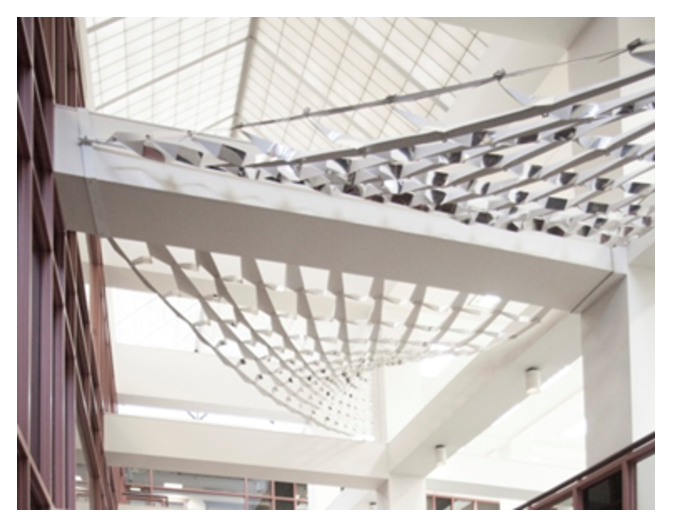
\includegraphics[width=0.5\linewidth]{figures/amp}
\label{fig:amp}}
\qquad \qquad
\subfloat[\mbox{ }]{
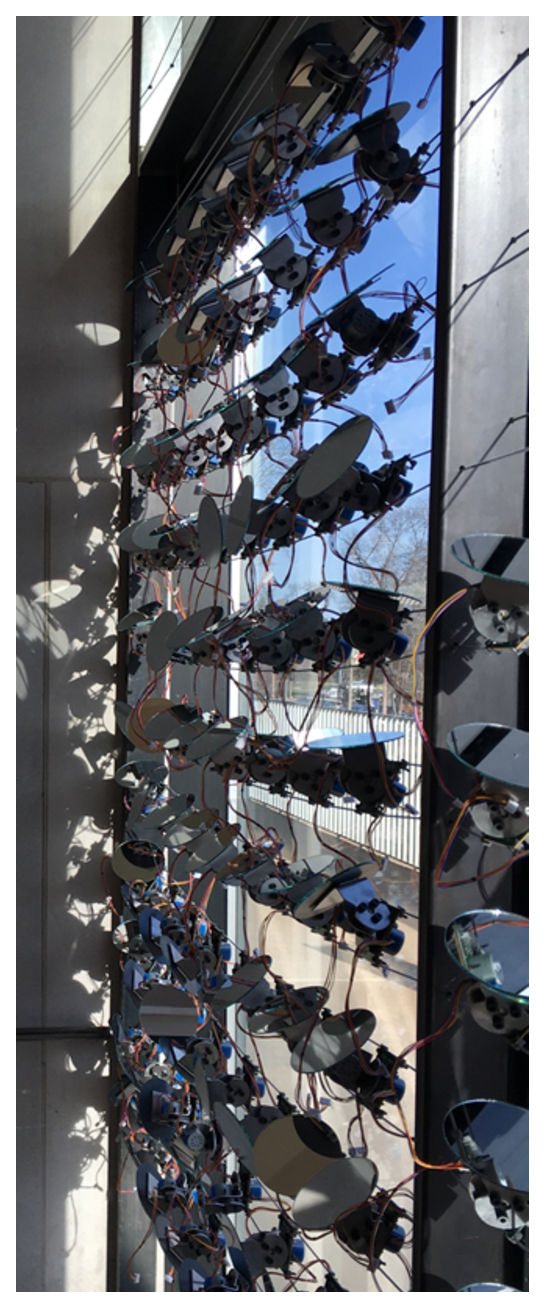
\includegraphics[width=0.16\linewidth]{figures/steinberg}
\label{fig:steinberg}}
\caption{Catoptric system prototypes.
(a)~\emph{AMP}, TRex building, St. Louis, MO.
(b)~\FIXME{name?}, Steinberg Hall, St. Louis, MO.
}
\label{fig:proto}
\end{figure}

In the next generation of this system, which is currently under construction,
over 600 mirrors are under active, 2-axis, microprocessor-based control and
therefore can be pointed in different directions dynamically as desired
over time. This installation is on the south wall of the Steinberg Hall
atrium (on
the campus of Washington University in St. Louis), and a subset of the
mirrors are shown in Figure~\ref{fig:steinberg}.

The ability to actively control the dynamic position of each mirror provides
for unprecidented capacity to position the available natural light where
it is desired.  This can easily change over time, as the usage of the
physical space changes.

The proposed research advances the investigation of reflected light by
designing specific intensities in some areas and dissipated lighting
conditions in other areas according to pre-determined, yet adjustable,
image-based maps. The maps can consist of any raster image and generate the
target positions for the reflected light in a space.  The image is sampled
according to intensity (black to white) to determine the density
of target points where the higher the value, the denser the resulting
field of points. Using an image-based map allows users to visualize
zones of intensity in an interior space prior to the mirrors reflecting
the daylight. Any user is capable of supplying or creating the image
to be used for the map, thus encouraging user control and interaction with
the system. The engagement of any member of a community on the creation
of that image has an impact on the entire community~\cite{BS13} and
encourages dialog about the quality and quantity of light within their
environment. 

Given the desire to control natural light (sunlight) via a catoptric surface,
repurposing it for illumination and/or thermal management, a number of
cruicial cyber-physical system issues must be addressed.
This research will investigate the following questions:
\begin{enumerate}

\item \emph{What are the qualitative and quantitative benefits
that can be achieved for bulding daylighting and thermal management
through the use of catoptric systems?}

Issues within this question include the ability to articulate the benefits
and to quantify them effectively.  Clearly, we are in the domain
of multi-objective control, so the relationship between the competing
goals must also be articulated and quantified. We intend to investigate
the use of Markov Decision Processes (MDPs) as an approach to
the multi-objective control problem, recognizing that maximization
(of an objective function) in expectation is a robust way to acknowledge
the inherent uncertainty of future events (whether it be sunlight availability,
lighting demand, or any other effect that is stochastic in nature).

\item \emph{How do we provide for the safety, reliability, maintainability, and
continued efficacy of these systems?}

Even with an ideal multi-objective control system in place, the system as
a whole has limited usefulness if these additional requirements are not
dealt with in an effective way.  Initially, just consider the issue of
safety: highly concentrated sunlight aimed at a heat collector (important
when harvesting energy for thermal management purposes) can be quite harmful
if inadvertently aimed at humans. 

Each of these system-level requirements must ultimately be included within
the optimization problem formulation, either as constraints (e.g., for
safety) or as additional objectives (e.g., reliability and/or maintainability).
Fortunately, the MDP formalism is well suited to the addition of concerns
such as these (especially those with a stochastic nature, as reliability
and maintainability tend to be).

\item \emph{Can we design abstractions that encapsulate subsystems for
effective reuse?}

A pair of immediate possibilities come to mind. Separating the concerns
of low-level control (e.g., of mirror positions) and high-level system
management (how the available light resource should be allocated) is one
option.  The low-level control subsystem can be encapsulated into a reusable
component, applicable to any number of physical positioning applications.
Similarly, a high-level management system (e.g., based upon MDP theory)
could also be encapsulated in a resuable component, applicable to any
number of other stochastic optimization problems.
Ultimately, we would like to generalize the above into abstractions that can be
leveraged more broadly for arbitrary cyber-physical systems development.

\end{enumerate}

\FIXME{Brief description of who we are and what we've done.}

%\section{Background and Related Work}
\label{sec:background}

\FIXME{Describe first two installations.}

\begin{figure}[ht]
\centering
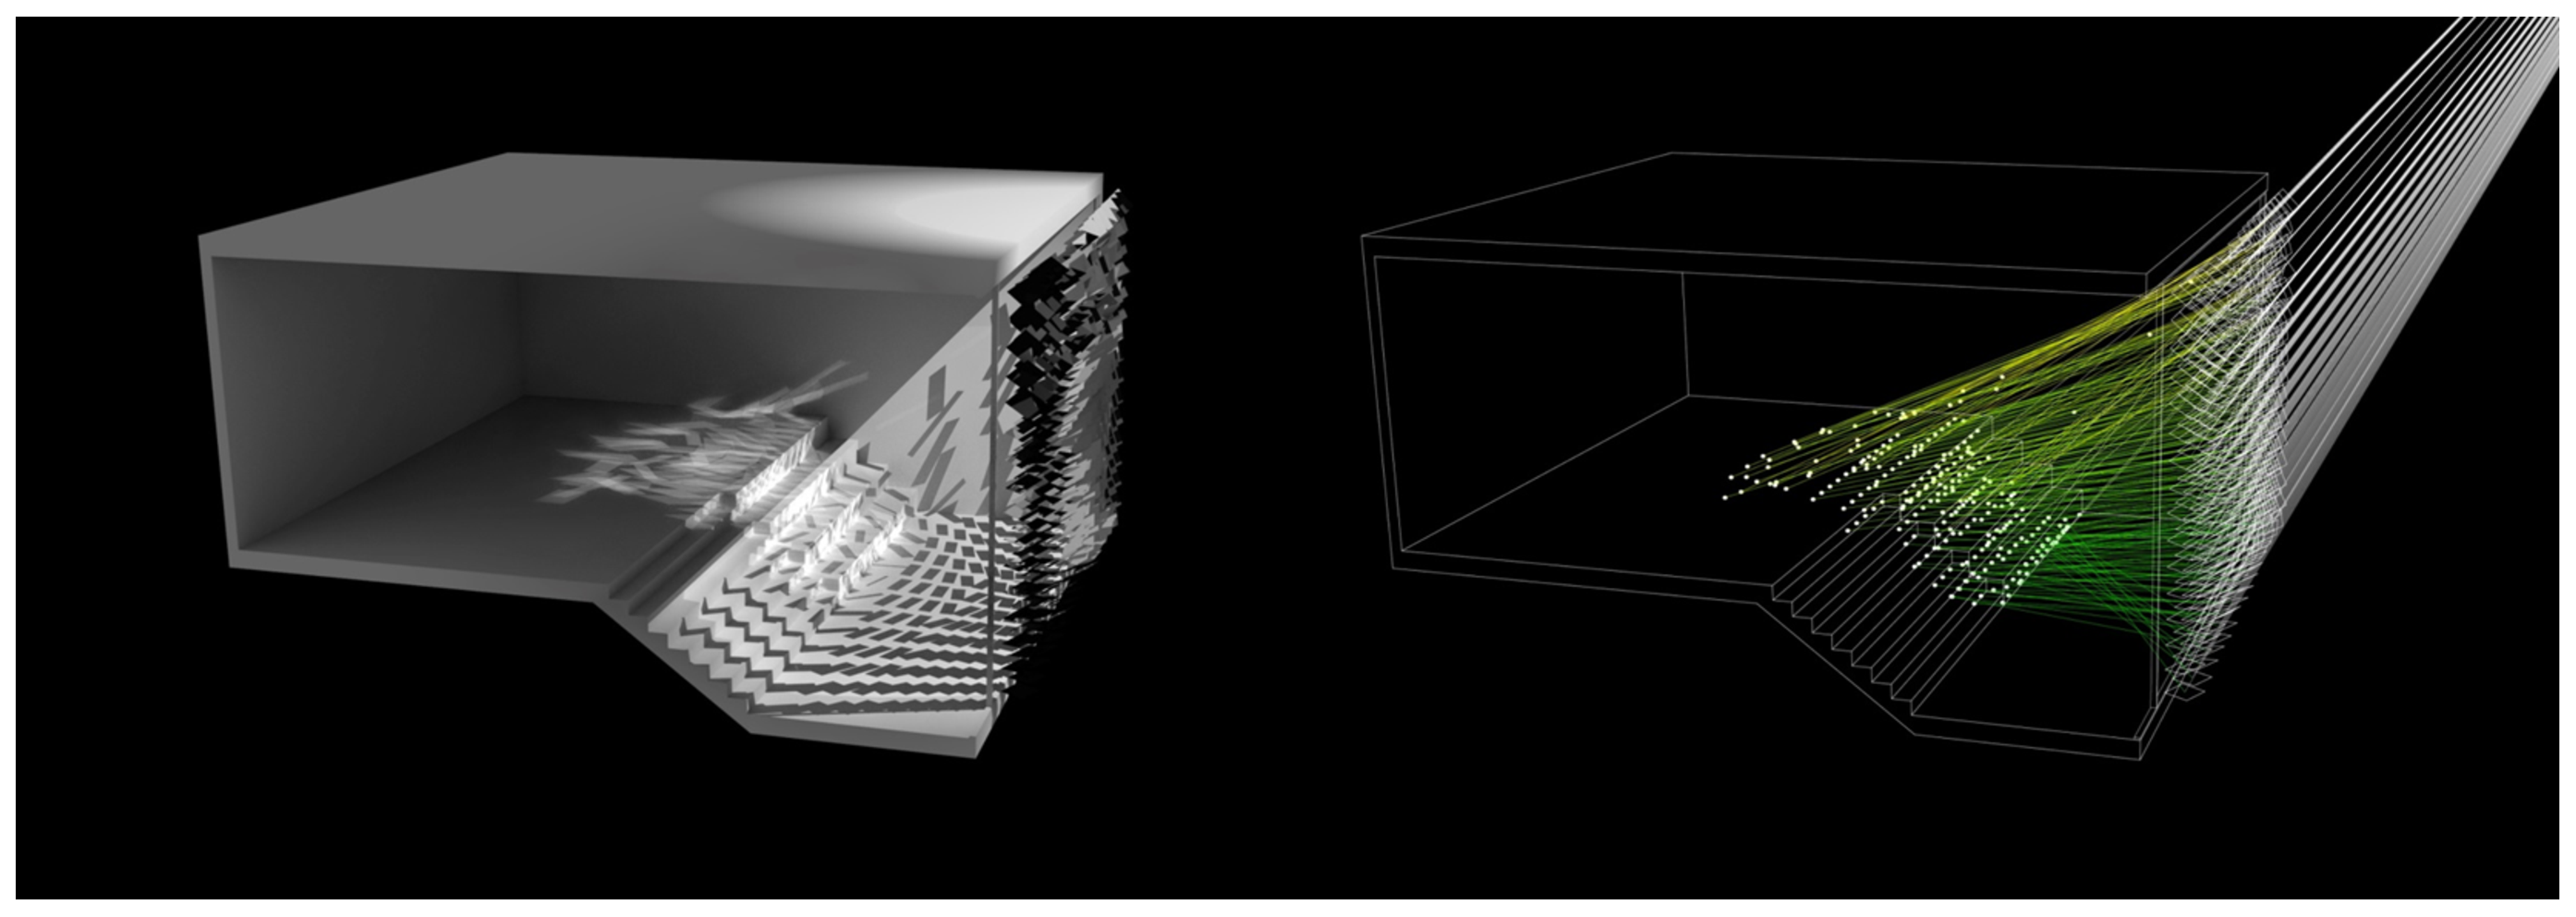
\includegraphics[width=0.8\linewidth]{figures/raytracing}
\label{fig:raytracing}
\caption{Ray tracing analysis of daylighting design.}
\end{figure}

Leslie~\cite{Leslie03} and Alrubaih et al.~\cite{azaise13} provide
a pair of review articles that effectively summarize the current
approaches to daylighting in modern building design.
For the most part, these are passive systems, or might include
active control of shades~\cite{kt16}, with a strong emphasis on
achieving uniform, homogeneous illumination~\cite{bwkk15,gb16}.
Our emphasis is on dynamic control of the light position, with the explicit
intent to be inhomogeneous in the illumination patterns.

There have been a number of efforts to quantitatively model and
empirically measure prototype daylighting
systems~\cite{bwkk15,fsdm14,ls06,vgf+13}. A pair of studies, first by
Lee and Selkowitz~\cite{ls06} and followed by Fernandes et al.\cite{fsdm14},
initially evaluated the potential for energy savings in the New York Times
Headquarters building and then measured the actual realized savings.

In this work, we will exploit Markov Decision Process (MDP)
formal theory~\cite{puterman} an an approach to optimization of the
catoptric surface control. MDPs represent a general approach
to modeling optimization problems and have been applied in a diverse set of
application areas~\cite{White93}. Examples include robotics~\cite{ab10}, 
economics~\cite{bs98}, experiment design~\cite{kb85},
medical decisions~\cite{ahsr10}, manufacturing~\cite{yyl04},
agriculture~\cite{Kristensen03},
and our own group's use in scheduling~\cite{gtsg08,tggs10}
and wireless spectrum management~\cite{mgc16}.

Our prior research has used Markov decision process
models~\cite{gtsg08} to generate resource management policies
off-line~\cite{gtgs09} for non-preemptive sharing of a resource
between multiple purposes at once on-line.  For example, a meter-tall robot's
camera (oriented by a pan-tilt unit similar to the ones we propose to
use in our multi-mirror catoptric installations) may be directed
downward to identify wire-frame chairs and other obstacles to
navigation that other sensors on the robot may have difficulty
detecting, or it may be directed upward to identify faces of people at
a reception whose images it can then capture. Given distributions of
the durations of intervals during which the camera would need to
remain pointed in a given direction to complete an individual task,
standard policy iteration techniques then can be used to generate
run-time policies that in expectation maximize an objective such as
adherence to a strictly proportional allocation of the resource over
time~\cite{gtsg08}, or even a more general definition of the utility 
of completing the different tasks at particular times~\cite{tggs10}.
We also showed that when different distributions of task completion
intervals can occur in different modes (e.g., when a robot moves
from room to room), it is possible to learn on-line what mode
the system is in, or if the mode is known what the distributions are,
but not both~\cite{gtgsuai10}.

However, policy iteration is exponentially expensive, and even the memory 
requirements to store complete policies for on-line use may be prohibitive 
in resource-limited systems.  We therefore focused next on the policies 
that were being generated from the models, and discovered consistent 
structure in those policies that allowed a reasonable heuristic 
approximation.  For simple proportional sharing, a single geometric partition
of a simplex could be calibrated to encode the appropriate policy accurately~\cite{gtspmgs10}.
For utility-based resource sharing multiple disjoint heuristics were needed but
the most effective one to use was clearly defined by problem parameters~\cite{tblwgs11}.

As a further illustration both of the applicability of MDP-based
policy iteration to generate effective resource management policies,
we applied similar techniques to manage a much different resource:
the transmission spectrum in wireless networks~\cite{mskgct13}.  Although 
the semantics of that resource differed radically from the pan-tilt camera, 
the MDP models were reasonably similar.  We extended the basic model to
include modulation as well as admission decisions, discovered and characterized
common structure among the policies that were generated, and again obtained
efficient and effective heuristic policies for on-line use~\cite{mgc16}.

In this proposal we adopt the definition used by Glaubius et al.~\cite{gtsg08}
of a (discrete-time) Markov decision process as a 5-tuple
$(\mathcal{X}, \mathcal{A}, T, R, \gamma)$, with \emph{states} designated
as $\chi \in \mathcal{X}$, \emph{actions} designated as $a \in \mathcal{A}$,
and a transition system, $T$, which gives the probability
$P_T (\chi' \mid \chi, a)$ of transitioning from state $\chi$ to
state $\chi'$ on action $a$.
The reward function $R(\chi, a, \chi') \in \mathbb R_{\ge 0}$ describes the
reward that accrues when transitioning from state $\chi$ to
state $\chi'$ via action $a$, under a discount factor, $\gamma$,
to ensure convergence of the long term reward.

\FIXME{Add transition into the next section.}

%\input{abstraction}
%\input{extensions}
%\input{tuning}
%\input{astro}
%\subsection{Intellectual Merit}
\label{sec:merit}

The main intellectual contributions of this proposed research entail
the development of new methods for multi-objective optimization of 
catoptric systems, i.e., rigorous techniques for deciding how a 
collection of controllable mirrors should be installed and how they 
should be positioned and (repositioned) from moment to moment.  We
will investigate not only the multi-objective control models,
policies, and mechanisms, but also issues of design for flexible
installation; ensuring safety, reliability, etc.; and exploring in
what ways catoptric systems can serve as a guiding example for more
general cyber-physical systems development.  Conducting these 
investigations will provide new insights into how MDP models can
be applied in cyber-physical-human contexts, the benefits and limitations
of doing so, and practical experience developing, evaluating, and operating
these systems.

%\section{Broader Impacts}
\label{sec:broader}

The proposed research is expected to have important impacts on the built environment.
According to the EPA, buildings are responsible for producing 6\% of
greenhouse gasses and heat and electrical generation produces another
25\%\footnote{\url{https://www.epa.gov/ghgemissions/global-greenhouse-gas-emissions-data}}.
A large portion of the electrical consumption in buildings is used for
heating, cooling and artificial lighting. Our proposal addresses the
reduction of electricity for artificial lighting to be replaced by
reflected daylight and capturing the solar heat. During daytime hours,
daylight is a preferred source of light for many people and the proposal
directs the daylight deeper into a building. The daylight reflection system
provides a more sustainable approach by reducing the required electricity
and provides a more desirable quality of light.

At the undergraduate level, this work is closely related to
our second-semester introductory course in computer science and
computer engineering.  The
text (co-authored by PI R. Chamberlain) is entitled {\it Computing
in the Physical World}~\cite{cc17}, and the course provides an introduction to
cyber-physical systems concepts in a laboratory-based setting.

The computational platform used in the course (an Arduino Uno) is the
same one used to control the Steinberg prototype catoptric surface,
and it has a very large hobbyist following (in the maker community).
We regularly request support for Research Experience for Undergraduate
(REU) students, and individuals who have completed
the above course will be well prepared to contribute to the research.

At the graduate education level, this work will support 4 graduate
students at Washington Univ.~in St.~Louis.
These students will be some combination of engineering students and
architecture students, with each community of students learning from
the other to broaden their individual horizons of experience to
include multidisciplinary work.

The Steinberg prototype was substantially designed by a student pursuing
dual degrees in architecture (MArch) and engineering (MEng)~\cite{Mitchell18}.
He recently gave an invited presentation to the Washington University Board
of Trustees about his experience, and the university is considering
a broader set of educational offerings that are tailored to students with
similar, cross-disciplinary interests.

We will leverage a pair of existing university programs to help us
attract students from traditionally underrepresented groups.  The Olin
Fellowship Program (for women) and the Chancellor's Fellowship Program
(aimed to recruit, support, and retain underrepresented minority 
students) have a successful track
record of enabling individuals to pursue graduate study.  In our
experience, the most effective method for attracting students from
underrepresented groups is by personal contact with a suitable role
model.  To facilitate this, we regularly ask the appropriately
qualified individuals in our group to be actively involved in the
recruiting process.  This cohort currently includes two
minority graduate students (one African-American student and one Hispanic 
student).
We will attempt to leverage the maker space community as one target
for broadening participation from traditionally underrepresented groups.

%\newpage
\section{Results from Prior NSF Support}
\label{sec:prior}

\noindent
{\large\bf CSR: Small: Concurrent Accelerated Data Integration}
{\bf (CNS-1527510,
PI R. Chamberlain, co-PI Ron Cytron)}, 
10/2015--9/2019, \$519,275.  

\textbf{Intellectual Merit} -- This project investigates the
accelerated execution of data integration workflows, which
increasingly are bottlenecks in data science. Execution platforms
being targeted include both graphics engines and FPGAs.

\textbf{Broader Impacts} -- This research project has supported 3
graduate students and 4 REU students.  The applications investigated
come from the fields of computational biology, astrophysics, and the
Internet of Things, further expanding the scope of the students'
experience.

\textbf{Evidence of Research Products and their Availability} --
Publications resulting from this work include~\cite{dibs,c17,mgc16,js16}.
A benchmark suite of the above workflows has been released
as a community resource~\cite{dibsv1}.

\noindent
{\large\bf CPS: Medium: Collaborative: CyberMech, a Novel Run-Time Substrate for 
Cyber-Mechanical Systems}
{\bf (CNS-1136073 and CNS-1136075,
Washington University: PI C. Gill, co-PIs Kunal Agrawal and Chenyang Lu; Purdue University: PI Arun Prakash, co-PI Shirley Dyke)}, 9/2011-8/2016, \$1,800,000 total.  

This research project developed novel foundations for parallel real-time computing, and used them to demonstrate the first ever real-time hybrid simulation involving a thousand-degree-of-freedom structure.

\textbf{Intellectual Merit} -- Results of this research include new methods for parallel real-time execution of control and simulation computations, new parallel real-time scheduling techniques and analyses, and characterization and exploitation of trade-offs involving both high computational demand and stringent timing constraints.

\textbf{Broader Impacts} -- This multi-university project involved 7 PhD, 3 masters, and 7 undergraduate students, and 2 visiting scholars in highly multi-disciplinary research collaborations.  Results of this research appeared in 10 publications at top-tier conferences and journals.

\textbf{Evidence of Research Products and their Availability} -- Data, experiment configurations, platform software, and simulation source-code have been published on-line at Washington University and Purdue University.

\begin{comment}
\vspace{0.1in}
\noindent
{\large\bf Very Energetic Radiation Imaging Telescope Array (VERITAS) Project}
{\bf (J. Buckley)}

This work was covered by a combination of a DOE research grant as well
as project funds in the form of DOE and NSF/Physics subcontracts
through the Smithsonian Astrophysical Observatory project office.

\textbf{Intellectual Merit} -- Significant products of the
work include the VERITAS FADC electronics and a number of scientific
results summarized in
\cite{2016MNRAS.461..202A,2016arXiv160901692A,2016arXiv160806464A,2016arXiv160801569A,2016MNRAS.459.2550A,2016ApJ...821..129A,2016ApJ...819..156B,2016ApJ...818L..33A,2016ApJ...817L...7A,2015ApJ...815L..22A,2015PhRvL.115u1103C,2015PhRvD..91l9903A,2015A&A...578A..22A,2015A&A...576A.126A,2015PDU.....7...16B,2015ApJ...800...61A,2015ApJ...799....7A,2014ApJ...797...89A,2014ApJ...795L...3A,2014ApJ...790..149A,2014ApJ...788..158A,2014ApJ...788...78A,2014ApJ...787..166A,2014ApJ...783...16A,2014ApJ...782...13A,2014APh....54....1A,2014arXiv1401.6085F,2014ApJ...780..168A,2013ApJ...779...92A,2013arXiv1310.8621A,2013arXiv1310.7040B,2013arXiv1310.5662B,2013ApJ...776...69A,2013arXiv1308.6173V,2013arXiv1307.4962P,2013arXiv1307.2807D,2013ApJ...770...93A,2013arXiv1305.0302W,2013arXiv1304.6367S,2013APh....43....3A,2013ApJ...764...38A,2013ApJ...762...92A}.
A founding member of VERITAS, Dr.\ Buckley was responsible for the design
and construction of the 2000-channel 500 Msps VERITAS FADC system.
He also played a leading role in establishing the scientific
programs for dark matter, multiwavelength studies of active galaxies
and observations of supernova remnants. Scientific highlights of
VERITAS include (1) DM limits on dwarf
galaxies\cite{2017PhRvD..95h2001A,2015PhRvD..91l9903A,2012PhRvD..85f2001A},
(2) resolved images and spectra from supernova remnants (SNR) leading
to direct evidence for the origin of hadronic cosmic rays in SNR
\cite{2017ApJ...836...23A,2013ApJ...764...38A,2013ApJ...770...93A,2010ApJ...719L..69A,2009ApJ...698L.133A},
(3) discovery of periodic emission from the Crab pulsar up to $>$100
GeV challenging current models of pulsar magnetospheres
\cite{2011Sci...334...69V}), (4) measurements of spectral variability
of active galaxies (AGNs) with multiwavelength data providing new
constraints on conditions near the central supermassive black hole
(e.g.,
\cite{2009ApJ...707..612A,2008ApJ...684L..73A,2011ApJ...726...43A,2009ApJ...691L..13D,2017ApJ...834....2A})
and (5) constraints on the extragalactic background light,
Lorentz-invariance violation and intergalactic magnetic fields
\cite{2012ApJ...750...94A,2010ApJ...708L.100A}.

\textbf{Broader Impacts} -- Information on VERITAS was disseminated to the
general public through YouTube videos, public site tours, and informational
displays at the Smithsonian Astrophysical Observatories. 

\textbf{Evidence of Research Products and their Availability} --

\end{comment}

%\input{conclude}

\clearpage
% \begin{scriptsize}
\bibliographystyle{abbrv}
%\bibliography{prop,wu,astro,refs}
\bibliography{prop}
% \end{scriptsize}

\end{document}
